\documentclass[ngerman]{article}
\usepackage{graphicx} % Für Bilder
\usepackage{adjustbox} % Für Rotationen und Skalierungen
\usepackage[a4paper,margin=2.5cm]{geometry} % Ränder setzen
\usepackage[ngerman]{babel} % Deutsche Spracheinstellungen
\usepackage{csquotes} % Korrekte Anführungszeichen
\usepackage{datetime} % Für deutsches Datum
\renewcommand{\dateseparator}{.} % Punkt als Datumstrenner
\usepackage{epstopdf} % Ermöglicht EPS-Nutzung mit pdflatex

\begin{document}

\title{Hausübung 2; UV WAP WS 2024/25}
\author{Gerwin Bacher \\
MatrNr: 12314104}
\date{24. Januar 2025}

\maketitle

\begin{figure}[ht]
    \centering
    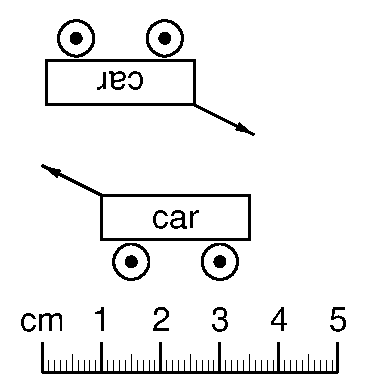
\includegraphics[width=0.8\textwidth]{car.eps}
    \caption{car.eps eingebunden in Latex}
    \label{fig:example_eps}
\end{figure}

\end{document}
